\subsection{Boundary points}

The number of integer points in the boundary of a polygon is:
$$ B = v + b $$
where v is the number of vertices (integer points as well) and b is the number of integer points situated between two vertices,
like in the following figure:

\begin{center}
  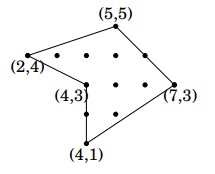
\includegraphics[scale=.6, keepaspectratio]{./theoretical/img/pick.png}
\end{center}

b can be calculated for every line connecting two points (including the line between the last and the first point) as follows:

$$
boundary\_points(p, q) = \begin{cases}
  |p.y - q.y| - 1 & $p.x = q.x$ \\
  |p.x - q.x| - 1 & $p.y = q.y$ \\
  gcd(|p.x - q.x|, |p.y - q.y|) - 1 \\
\end{cases}
$$